\documentclass{cumcm}


% \title{text}这里是显示在第三页的文章标题
\title{机场的出租车问题}
% \displaytitle{text} 这里是显示在承诺书上的文章标题,注意,不能换行,如果题目特别长,要进行适当的缩写
\displaytitle{机场的出租车问题}
% \school{text}命令用于在承诺书上显示学校名称。按要求,此处应填写全称
\school{上海交通大学}
% 以下命令分别显示队员、指导教师姓名以及队伍编号
\authorone{刘畅}
\authortwo{谢哲}
\authorthree{胡胜超}
\advisor{}
\teamnumber{未知报名号}
\dateyear{2019}
\datemonth{9}
\dateday{7}

\begin{document}

% 这里用于打印承诺书以及编号页
 
%\newpage
\thispagestyle{empty} %取消当前页码
{\Large \heiti \begin{center}\the\year~高教社杯全国大学生数学建模竞赛\par\vspace{0.5\ccwd}\par
{\ziju{1}承诺书}\end{center}\par\vspace{1\ccwd}\par}
\renewcommand{\baselinestretch}{1.5}\normalsize
{\zihao{-4}%
我们仔细阅读了中国大学生数学建模竞赛的竞赛规则。\par
我们完全明白,在竞赛开始后参赛队员不能以任何方式(包括电话、电子邮件、网上咨询等)
与队外的任何人(包括指导教师)研究、讨论与赛题有关的问题。\par
我们知道,抄袭别人的成果是违反竞赛规则的, 如果引用别人的成果或其他公开的资料
(包括网上查到的资料),必须按照规定的参考文献的表述方式在正文引用处和参考文献中明确列出。\par
我们郑重承诺,严格遵守竞赛规则,以保证竞赛的公正、公平性。如有违反竞赛规则的行为,我们将受到严肃处理。\par
\par\vspace{2\ccwd}\par
\raisebox{1ex}[0pt]{我们参赛的题目是:}\vbox{\hbox to11.4cm{\hfil \the\displaytitle \hfil}
        \protect\vspace{0.6truemm}\relax
        \hrule depth0pt height0.15truemm width11.4cm}\par
\vspace{1mm}
\raisebox{1ex}[0pt]{我们的参赛报名号为(如果赛区设置报名号的话):}\vbox{\hbox to5.75cm{\hfil \the \teamnumber  \hfil}
        \protect\vspace{0.6truemm}\relax
        \hrule depth0pt height0.15truemm width5.75cm}\par
\vspace{1mm}
\raisebox{1ex}[0pt]{所属学校(请填写完整的全名):}\vbox{\hbox to9.12cm{\hfill \the\school \hfill}
        \protect\vspace{0.6truemm}\relax
        \hrule depth0pt height0.15truemm width9.12cm}\par
\begin{tabular}{lcp{8.82cm}c}
\hspace{-2.1mm}\raisebox{-1mm}[0pt]{参赛队员(打印并签名): }&\raisebox{-1mm}[0pt]{1、}& \raisebox{-1mm}[0pt]{\the\authorone\hfill{}}& \\ \cline{3-3}
   &\raisebox{-1mm}[0pt]{2、}& \raisebox{-1mm}[0pt]{\the\authortwo\hfill{}}& \\ \cline{3-3}
   &\raisebox{-1mm}[0pt]{3、}& \raisebox{-1mm}[0pt]{\the\authorthree\hfill{}}& \\ \cline{3-3}
\end{tabular}
\par
\vspace{10mm}
\raisebox{1ex}[0pt]{指导教师或指导教师组负责人(打印并签名):}\vbox{\hbox to6.65cm{\the\advisor \hfil}
        \protect\vspace{0.6truemm}\relax
        \hrule depth0pt height0.15truemm width6.65cm}\par
\vspace{5mm}
{}\hspace{10cm}日期:\uline{\hspace{0.5em}\the\dateyear\hspace{0.5em}}年\uline{\hspace{0.5em}\the\datemonth\hspace{0.5em}}月 
\uline{\hspace{0.5em}\the\dateday\hspace{0.5em}}  日
\par
\vspace{2cm}
\hrulefill\par\vspace{2\ccwd}\par
赛区评阅编号(由赛区组委会评阅前进行编号):
}
\renewcommand{\baselinestretch}{1.3}\normalsize
\newpage
\thispagestyle{empty} %取消当前页码
{\Large \heiti \begin{center}\the\year~高教社杯全国大学生数学建模竞赛\par\vspace{0.5\ccwd}\par
{\ziju{1}编号专用页}\end{center}\par\vspace{1\ccwd}\par}
{\zihao{-4}%
\par\vfill
赛区评阅编号(由赛区组委会评阅前进行编号):\par\vfill\vfill

赛区评阅记录(可供赛区评阅时使用):\vspace{1\ccwd}

\begin{center}
\resizebox{.9\textwidth}{!}{
\begin{tabular}{|c|*{10}{p{.09\textwidth}|}}
\hline
\makecell{评\\阅\\人}&&&&&&&&&&\\
\hline
\makecell{评\\分}&&&&&&&&&&\\
\hline
\makecell{备\\注}&&&&&&&&&&\\
\hline
\end{tabular}
}
\end{center}\vspace{1\ccwd}

全国统一编号(由赛区组委会送交全国前编号):\par\vfill\vfill

全国评阅编号(由全国组委会评阅前进行编号):\par\vfill\vfill\vfill
}
\renewcommand{\baselinestretch}{1.3}\normalsize

\newpage

\begin{minipage}{0.9\textwidth}
\centering\LARGE\textbf{机场的出租车问题}
\end{minipage}

% 摘要和关键字
\begin{abstract}
	摘要部分,是文章最为重要的部分之一,一般放在最后来写。
	引用一些参考文献\cite{citetest}。首先简要概括一下题目。\par
	\textbf{针对问题一}\quad
	对问题一的解答的概括。\par
	\textbf{针对问题二}\quad
	对问题二的解答的概括。\par
	\textbf{针对问题三}\quad
	对问题三的解答的概括。
\\\par
\textbf{关键词\quad MATLAB\quad \LaTeX}
\end{abstract}

\newpage
\section{问题重述}
\subsection{问题背景}
出租车是乘客往返市区与机场的主要交通方式之一。机场有客流密度大的特点,而乘客需要在固定的出租车上客点乘车。由于上客点地点和条件有限,且上客的效率受到了乘客、机场航班、出租车司机等多种因素的影响。所以需要一种优化的解决方案能够提高乘客在出租车上客点的乘车效率,以减少乘客和出租车司机的等待时间。
\subsection{问题重述}
国内机场一般将出租车乘车区分为上客区和下客区两个分开的区域,并且对于离开上客区的出租车,司机可以根据的意愿选择放空车辆直接离开或前往“蓄车池”载客。对于司机,他们可以得到当前“蓄车池”内的车的数量以及当前的航班数量来决定是否进入“蓄车池”等待,并且司机通常还可以根据自己的经验,结合季节、时间等因素判断乘客数量的多少。对于机场管理者,他们需要在上客地点的等候区采取“分批定量”放行的措施来让乘客依次进入上客区乘车。\par
\begin{figure}[H]
	\centering
	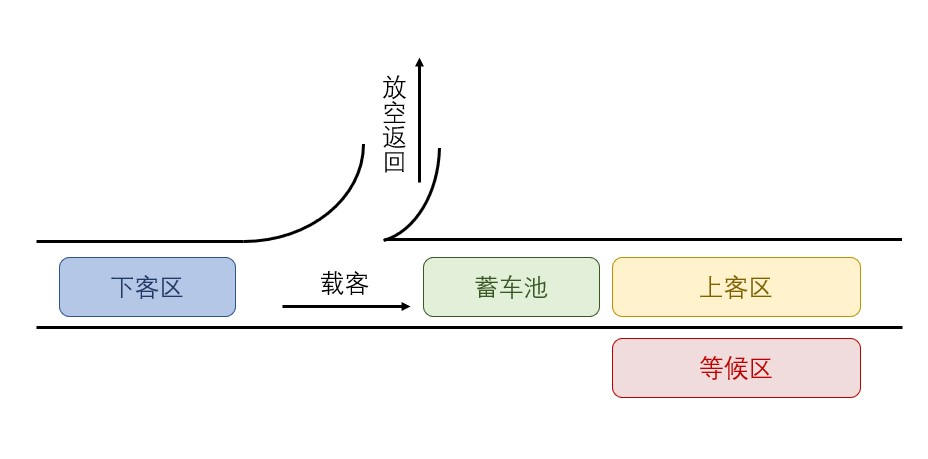
\includegraphics[width=0.8\textwidth]{img/taxi_example.jpg}
	\caption{机场出租车乘车区域示意图}
	\label{taxi_example}
\end{figure}
根据以上条件,我们需要研究如下的4个问题:
\begin{enumerate}[(1)]
	\item 建立一个模型,用于出租车司机载客与放空返回的选择策略。建立模型时综合考虑机场在不同时间的旅客数量的变化规律和其它的相关因素,使得出租车的做出的策略能够使其收益最大化。
	\item 获取国内某一机场的实际数据,根据建立的模型和机场的实际数据计算出司机的决策策略,并由此可以出模型的合理性与对相关因素的依赖程度。
	\item 机场乘车区设置有两条并行车道,建立一个模型,确定合理的“上车点”的位置,与出租车和乘客的安排方式,在确保安全的前提下,使得出租车和乘客的乘车效率能够最大化。
	\item 出租车在机场载客的目的地不确定,且司机无法自主选择载客或拒绝载客,故司机的收益不确定。为了解决这个问题,考虑给予返回的短途载客的司机在下一次载客时的优先权。建立一个模型,给出可行的优化方案,使得出租车司机们的收益能够尽可能均衡。
\end{enumerate}

\section{模型假设}
\begin{enumerate}
	\item 一些不切实际的假设。
	\item 另一些不现实的假设。
\end{enumerate}
\section{符号说明}
表\ref{table-symbol}列出了本文需要的符号。
\begin{table}[H]
	\centering
	\caption{符号说明} 
	\label{table-symbol}
	\begin{tabular*}{0.3\textwidth}{ccc}
		\toprule
		\multirow{2}{*}{符号} & a & b \\
		\cline{2-3}
		
		& b & c\\
		\midrule
		$\rho$ & 海水的密度 & $kg/m^3$ \\
		\bottomrule
	\end{tabular*}
\end{table}

\section{问题分析}
\subsection{问题一的分析}
分析问题的本质,并且给出解决这个问题的基本步骤。

\subsection{问题二的分析}

\subsection{问题三的分析}

\section{模型建立}
建立模型的数学推导和相关图示。

\section{问题解答}
问题的具体解答过程,和解答过程中使用算法的伪代码。和最终计算出来的解答结果。

\section{模型总结}
\subsection{模型优点}
\begin{enumerate}
	\item 把模型的有点一一列举出来。
\end{enumerate}

\subsection{模型缺点}
\begin{enumerate}
	\item 把模型的缺点一一列举出来。
\end{enumerate}

\bibliographystyle{plain}
\bibliography{ref}

\newpage
\appendix
\textbf{附录}
\section{模型代码}
\subsection{问题一代码}
\begin{lstlisting}
	% 这里放置代码
\end{lstlisting}
\end{document}